% !TEX encoding = UTF-8 Unicode
\documentclass[
10pt,
aspectratio=169,
]{beamer}
\setbeamercovered{transparent=10}
\usetheme[
%  showheader,
%  red,
  purple,
%  gray,
%  graytitle,
  colorblocks,
%  noframetitlerule,
]{Verona}

\usepackage[T1]{fontenc}
\usepackage[utf8]{inputenc}
\usepackage{lipsum}
%%%%%%%%%%%%%%%%%%%%%%%%%%%%%%%
% Mac上使用如下命令声明隶书字体,windows也有相关方式,大家可自行修改
%\providecommand{\lishu}{\CJKfamily{zhli}}
%%%%%%%%%%%%%%%%%%%%%%%%%%%%%%%
\usepackage{tikz}
\usetikzlibrary{fadings}
\usetikzlibrary{shapes.geometric}
\usetikzlibrary{positioning}
%\tikzset{
%  every overlay node/.style={
%    draw=black,fill=white,rounded corners,anchor=south west,
%  },
%}
% Usage:
% \tikzoverlay at (-1cm,-5cm) {content};
% or
% \tikzoverlay[text width=5cm] at (-1cm,-5cm) {content};
%\def\tikzoverlay{%
%   \tikz[baseline,overlay]\node[every overlay node]
%}%
\tikzset{
  every overlay node/.style={
    anchor=north west,
  },
}
\def\tikzoverlay{%
   \tikz[baseline,overlay]\node[every overlay node]
}%


\newenvironment{smallgreentext}{\scriptsize\color{green}}{\par}
\newenvironment{smallbluetext}{\scriptsize\color{blue}}{\par}
\def\checkmark{\tikz\fill[scale=0.4](0,.35) -- (.25,0) -- (1,.7) -- (.25,.15) -- cycle;}

%
%\setbeamertemplate{sections/subsections in toc}[ball]
%\usepackage{xeCJK}
\usepackage{adjustbox} % Shrink stuff
\usepackage{listings}
\usepackage{caption}
\usepackage{subcaption}
\usefonttheme{professionalfonts}
\def\mathfamilydefault{\rmdefault}
\usepackage{amsmath}
\usepackage{multirow}
\usepackage{booktabs}
\usepackage{bm}
\setbeamertemplate{section in toc}{\hspace*{1em}\inserttocsectionnumber.~\inserttocsection\par}
\setbeamertemplate{subsection in toc}{\hspace*{2em}\inserttocsectionnumber.\inserttocsubsectionnumber.~\inserttocsubsection\par}
\setbeamerfont{subsection in toc}{size=\small}
\AtBeginSection[]{%
	\begin{frame}%
		\frametitle{Outline}%
		\textbf{\tableofcontents[currentsection]} %
	\end{frame}%
}

\AtBeginSubsection[]{%
	\begin{frame}%
		\frametitle{Outline}%
		\textbf{\tableofcontents[currentsection, currentsubsection]} %
	\end{frame}%
}

\title{Propuesta: t\'itulo y objetivos}
\subtitle{Estructuraci\'on y realizaci\'on de la propuesta}
\author[L.M.]{Luis Alejandro Morales, Ph.D.}
\mail{lmoralesm@unal.edu.co}
\institute[UNAL]{Facultad de Ingenier\'ia, Departamento de Ingnenier\'ia Civil y Agr\'icola\\
Universidad Nacional de Colombia, Bogot\'a}
\date{\today}
\titlegraphic[width=3cm]{logo_01u}{}

%%%%%%%%%%%%%%%%%%%%%%%%%%%%%%%%
% ----------- 标题页 ------------
%%%%%%%%%%%%%%%%%%%%%%%%%%%%%%%%
% New commands
\newcommand{\gi}{\texttt{Git}}
\newcommand{\gih}{\texttt{GitHub}}
\newcommand{\co}[1]{\alert{\textbf{\large \texttt{#1}}}}

\begin{document}

\maketitle

%%% define code
\defverbatim[colored]\lstI{
	\begin{lstlisting}[language=C++,basicstyle=\ttfamily,keywordstyle=\color{red}]
	int main() {
	// Define variables at the beginning
	// of the block, as in C:
	CStash intStash, stringStash;
	int i;
	char* cp;
	ifstream in;
	string line;
	[...]
	\end{lstlisting}
}
%%%%%%%%%%%%%%%%%%%%%%%%%%%%%%%%
% ----------- FRAME ------------
%%%%%%%%%%%%%%%%%%%%%%%%%%%%%%%%

%----
\section{Titulo}
\begin{frame}{Titulo}
El titulo debe reflejar y ser congruente con el \alert{objetivo principal}. El t\'itulo debe cumplir dos funciones:
\begin{itemize}
\item \alert{Atraer} a otros para leer el documento
\item Proporcionar la \alert{mejor información posible} para, e.j. agilizar la búsqueda
\end{itemize}
\emph{¿Como construir un buen titulo?}
\begin{enumerate}
\item Escoger las \alert{palabras claves} en su proyecto.
\item Ordenar las palabras claves de acuerdo con su \alert{importancia}.
\item Construya el titulo colocando las \alert{palabras} de acuerdo con el \alert{orden de importancia}.
\item Si el titulo es \alert{muy largo}, \alert{borre} las palabras menos importantes. 
\end{enumerate}
\tikzoverlay[text width=12cm] at (1cm,0.5cm) {
\begin{smallgreentext}
The influence of season of calving on the performance of Holstein cows.
\end{smallgreentext}
\begin{smallbluetext}
Holstein cows produce more milk if they calve in spring instead of autumn. \checkmark
\end{smallbluetext} 
};
\end{frame}

\begin{frame}{Ejercicio}
Lea al menos 3 t\'itulos de art\'iculos relacionados con su tema de investigaci\'on y establezca si se cumple lo anterior.
\end{frame}

\section{Objetivos}

\begin{frame}{Introducci\'on: The topdown approach}
\tikzoverlay[text width=1.5cm] at (2.3cm,2cm) {
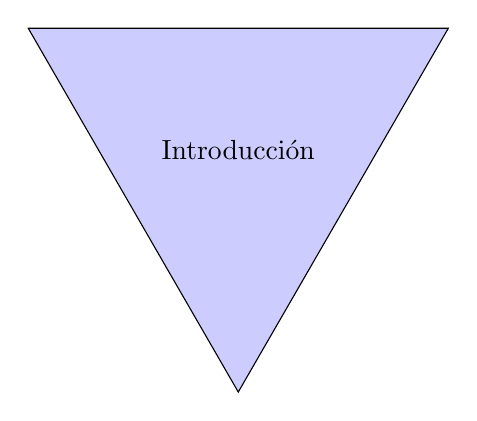
\begin{tikzpicture} 
% \node[regular polygon,regular polygon sides=3, draw, fill=blue!20, shape border rotate=180] at (-4cm,0){Introducci\'on};
 \node[regular polygon,regular polygon sides=3, draw, fill=blue!20, shape border rotate=180] at (current page.center){Introducci\'on};
\end{tikzpicture}
};
\tikzoverlay[text width=4.5cm] at (8.3cm,2cm) {
\alert{What is the status quo?}
};
\tikzoverlay[text width=4.5cm] at (8.3cm,0cm) {
\alert{What is wrong with the status quo?}
};
\tikzoverlay[text width=4.5cm] at (8.3cm,-2cm) {
\alert{\textbf{How does my project/paper go beyond the status quo?}}
};
\end{frame}

\begin{frame}{Objetivos: generalidades}
\begin{itemize}
\item Los objetivos de un proyecto de investigación resumen lo que se puede lograr mediante el estudio y deben estar estrechamente relacionados con el planteamiento del problema.
\item Los objetivos de la investigación se derivan del propósito. Establecen lo que se debe lograr en una investigación en términos específicos.
\item Son cruciales en cualquier investigación ya que determinan el tipo de preguntas y procedimientos que se utilizarán en, por ejemplo, la obtención y análisis de datos, diseño de experimentos, etc.
\item Al establecer los objetivos, se deben utilizar verbos imparciales como: \alert{determinar}, \alert{encontrar}, \alert{investigar}, \alert{examinar}, \alert{explorar}, \alert{establecer}, \alert{diferenciar}, \alert{comparar}, \alert{comprobar}, etc.
\end{itemize}
\end{frame}

\begin{frame}{Objetivos: generalidades}
Al formular objetivos, se debe tener cuidado específicamente con:
\begin{enumerate}
\item Asegurarse de que los objetivos sean claros, bien escritos y precisos.
\item Hacer que los objetivos sean específicos, significativos, realistas y realizables.
\item Asegurarse que los objetivos fluyan lógicamente desde la declaración de necesidad,  y que aborden el problema.
\item Hacer que los objetivos se encuentren dentro del alcance de los resultados que se espera alcanzar dentro del límite de tiempo, dinero y recursos disponibles.
\item Establecer los objetivos, en la medida de lo posible, en términos que permita medir o observar su realizaci\'on.
\item Los objetivos deben ser jerárquicos y/o cronológicos y/o tem\'aticos. 
\end{enumerate}
\end{frame}

\begin{frame}{Objetivos}
\begin{itemize}
\item \alert{Objetivo general}: Establece lo que se espera lograr mediante el estudio en términos generales.
\item \alert{Objetivos espec\'ificos}
\begin{itemize}
\item Partes más pequeñas y lógicamente conectadas que se derivan del objetivo general.
\item Son los aspectos específicos de el tema que queremos estudiar y/o resolver en el marco de nuestro estudio.
\item Los objetivos específicos deben abordar sistemáticamente varios aspectos del problema y los factores clave que se supone que influyen o causan el problema.
\item Deberían especificar \alert{qué haremos} en nuestro estudio, \alert{dónde} y con qué \alert{propósito}.
\end{itemize}
\end{itemize}
\end{frame}

\begin{frame}{Objetivos: Ejemplo}
\begin{center}
\textbf{Implementaci\'on y evaluaci\'on de un modelo matem\'atico para el transito bidimensional de una onda de creciente en el sector del Canal del Dique en el R\'io Magdalena}
\end{center}
\begin{itemize}
\item \alert{Objetivo general}: Implementar y evaluar un modelo m\'atematico para la simulaci\'on bidimensional del transito de una onda de creciente en el sector del Canal del Dique en el R\'io Magdalena. 
\end{itemize}

\end{frame}

\begin{frame}{Objetivos: Ejemplo}
\footnotesize
\begin{itemize}
\item \alert{Objetivos espec\'ificos}
\begin{itemize}
\footnotesize
\item Describir matem\'atica y f\'isicamente el sistema de ecuaciones diferenciales parciales hiperbólicas, que gobiernan el flujo bidimensional no permanente en canales.
\item Caracterizar hidr\'aulicamente las secciones del R\'io Magdalena en el sector de la derivaci\'on del Canal del Dique, con el fin de determinar su geometr\'ia, coeficientes de rugosidad del lecho y las orillas, regimenes de flujo y condiciones fisicas de contorno.
\item Analisar y comparar algunos modelos num\'ericos en diferencias finitas utilizados para la soluci\'on de las ecuaciones que rigen el fen\'omeno, con el fin de determinar las ventajas y desventajas de cada uno de ellos.
\item Establecer las condiciones iniciales y de frontera del sistema, para la soluci\'on de las ecuaciones de flujo bidimensional. 
\item Construir y programar un modelo matem\'atico para la simulaci\'on del flujo bidimensional no permanente en canales. 
\item Evaluar y validar num\'ericamente el modelo mediante la simulaci\'on de casos comúnmente estudiados como el rompimiento de presas, calculo de flujo transcr\'itico y transito de crecientes en canales prism\'aticos.
\item Calibrar el modelo matem\'atico para el caso de la simulaci\'on de crecientes en el sector de la derivaci\'on del Canal del Dique en el R\'io Magdalena, con base en la informaci\'on hidrom\'etrica de las estaciones ubicadas en la zona.
\item Validar el modelo mediante la comparaci\'on con series temporales de caudal y nivel, medidas en las secciones de frontera ubicadas aguas abajo en el sector. 
\end{itemize}
\end{itemize}

\end{frame}

\begin{frame}{Ejercicio}
De un art\'iculo de inter\'es del tema de investigaci\'on, indentif\'ique el objetivo general y los objetivos espec\'ificos.
\end{frame}

\end{document}


